\documentclass[a4paper]{article}

\usepackage{graphicx,url,a4wide}
\usepackage[french]{babel}
\usepackage{color}       % bold math

\begin{document}

\begin{center}{\Large \bf
Algorithme du firmware}

{C. Droit, \today}%
\end{center}

%\begin{abstract}

%\end{abstract}

\section{Introduction}
Voici un aper\c cu de l'algorithme du firmware



\section{Explication de la fonction main (Fig. \ref{hw1})}
Le menu pricipal ``main'' est le corp du programme, il va de l'initialisation \`a l'affichage des donn\'ees en passant par l'appel des
fonctions. 
\begin{itemize}
\item M1 $\rightarrow$ Calcul du pas de fr\'equence en fonction de Fintsta et Fintsto (Fig. \ref{hw3})
\item M2 $\rightarrow$ L'interrogation est s\'epar\'ee en deux parties, une interrogation des capteurs de pression puis des capteurs de temp\'erature
 (interrogation + affichage des donn\'ees). Pour avoir un affichage valide de la fr\'equence de r\'esonance, l'interrogateur doit voir soit tous les 
capteurs de pression ou tous les capteurs de temp\'erature. Dans le cas ou nous activons le mode tracking, si l'interrogateur ne voit plus un capteur 
de pression, il passe en interrogation peigne fixe sans perturber le mode tracking sur les capteurs de temp\'erature.
\end{itemize}


\section{Explication fonction balaie\_ ism (Fig. \ref{hw2})}
La fonction balaie\_ ism est la fonction permettant l'interrogation, elle va g\'erer l'\'emission de fr\'equence, la r\'eception et 
le traitement de la mesure, et le calcule de la fr\'equence de r\'esonance.
\begin{itemize}
\item B1 $\rightarrow$ En fonction du mode activ\'e mode ``tracking'' ou ``peigne fixe'' avec la variable ``mode\_ balaye\_ continu'', l'ex\'ecution 
du programme passe par la localisation de la fr\'equence de r\'esonance une premi\'ere foi pour pouvoir calculer la nouvelle fen\^etre d'interrogation 
qui sera utilis\'ee lors du prochain passage dans la fonction. Soit le mode tracking est activ\'e et l'ex\'ecution passe pas B1 ou nous allons directement 
\`a la partie B5.
\item B2 $\rightarrow$ La boucle de r\'ep\'etition permet l'accumulation de NBMOY mesure pour calculer la variance et la moyenne des fr\'equences 
de r\'esonances trouv\'ees.
\item B3 $\rightarrow$ Le traitement de la mesure permet avoir la moyenne des fr\'equences de r\'esonances trouv\'ees et la variance sur ces fr\'equences, 
ce qui permet de juger si la mesure r\'ealis\'ee est bonne ou fausse.
\item B4 $\rightarrow$ Nous retournons 100 + total si nous avons r\'eussi \`a avoir NBMOY mesure, la variable ``total``  est le nombre 
d'interrogation effectu\'ee. Sinon, nous retournons BSP (le nombre mesure acquise et valide).
\item B5 $\rightarrow$ Si nous avons choisi le mode peigne fixe, nous arrivons directement dans cette partie de la fonction. Sinon si le mode tracking 
est choisi, nous avons d\'eja \'effectu\'e le premier balayage qui nous a permit d'ajuster la fen\^etre d'interrogation.
\item B6 $\rightarrow$ En mode tracking, si nous ne trouvons pas la fr\'equence de r\'esonance dans les points acquis, nous agrandissons la fen\^etre 
d'interrogation tant que nous n'avons pas la fr\'equence de r\'esonance. Nous avons ajout\'e un d\'elai avant de l'agrandir pour \'eviter de sortir trop 
vite du mode tracking. La fen\^etre d'interrogation ne peut \^etre plus grande que les fr\'equences limites que nous avons rentr\'e (Finsta, Finsto). 
Dans le cas ou nous ne trouvons pas de fr\'equence de r\'esonance, nous retournons que nous avons pas trouv\'e de fr\'equence de r\'esonance (bsp=0)
 et une variance de 100000 + le num\'ero du r\'esonateur l'interrogateur n'a pas trouv\'e. Avec une grande variance, nous pouvons \'eliminer la mesure quand nous l'afficherons dans l'interface graphique.
\end{itemize}

\begin{figure}[h!tb]
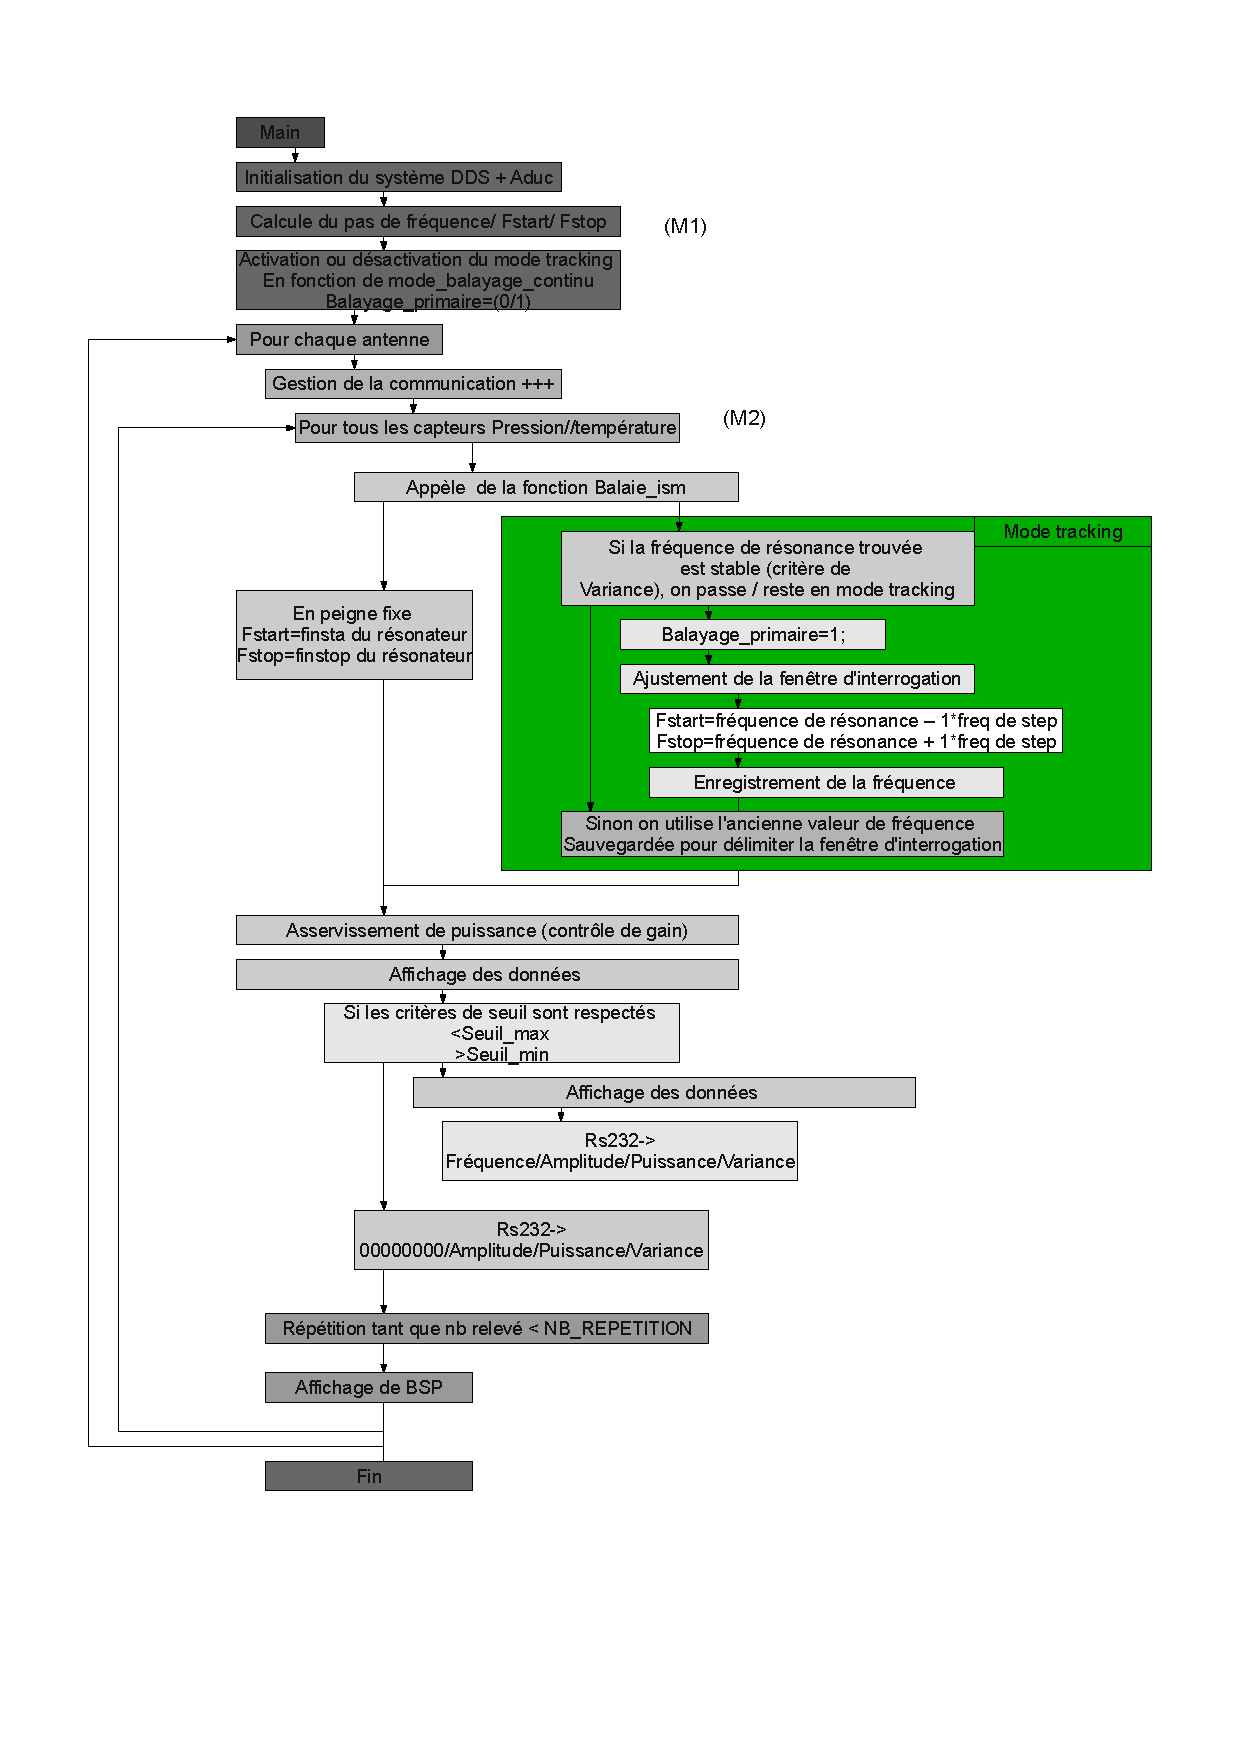
\includegraphics[width=\linewidth]{algo}
\caption{Menu principal}
\label{hw1}
\end{figure}

\begin{figure}[h!tb]
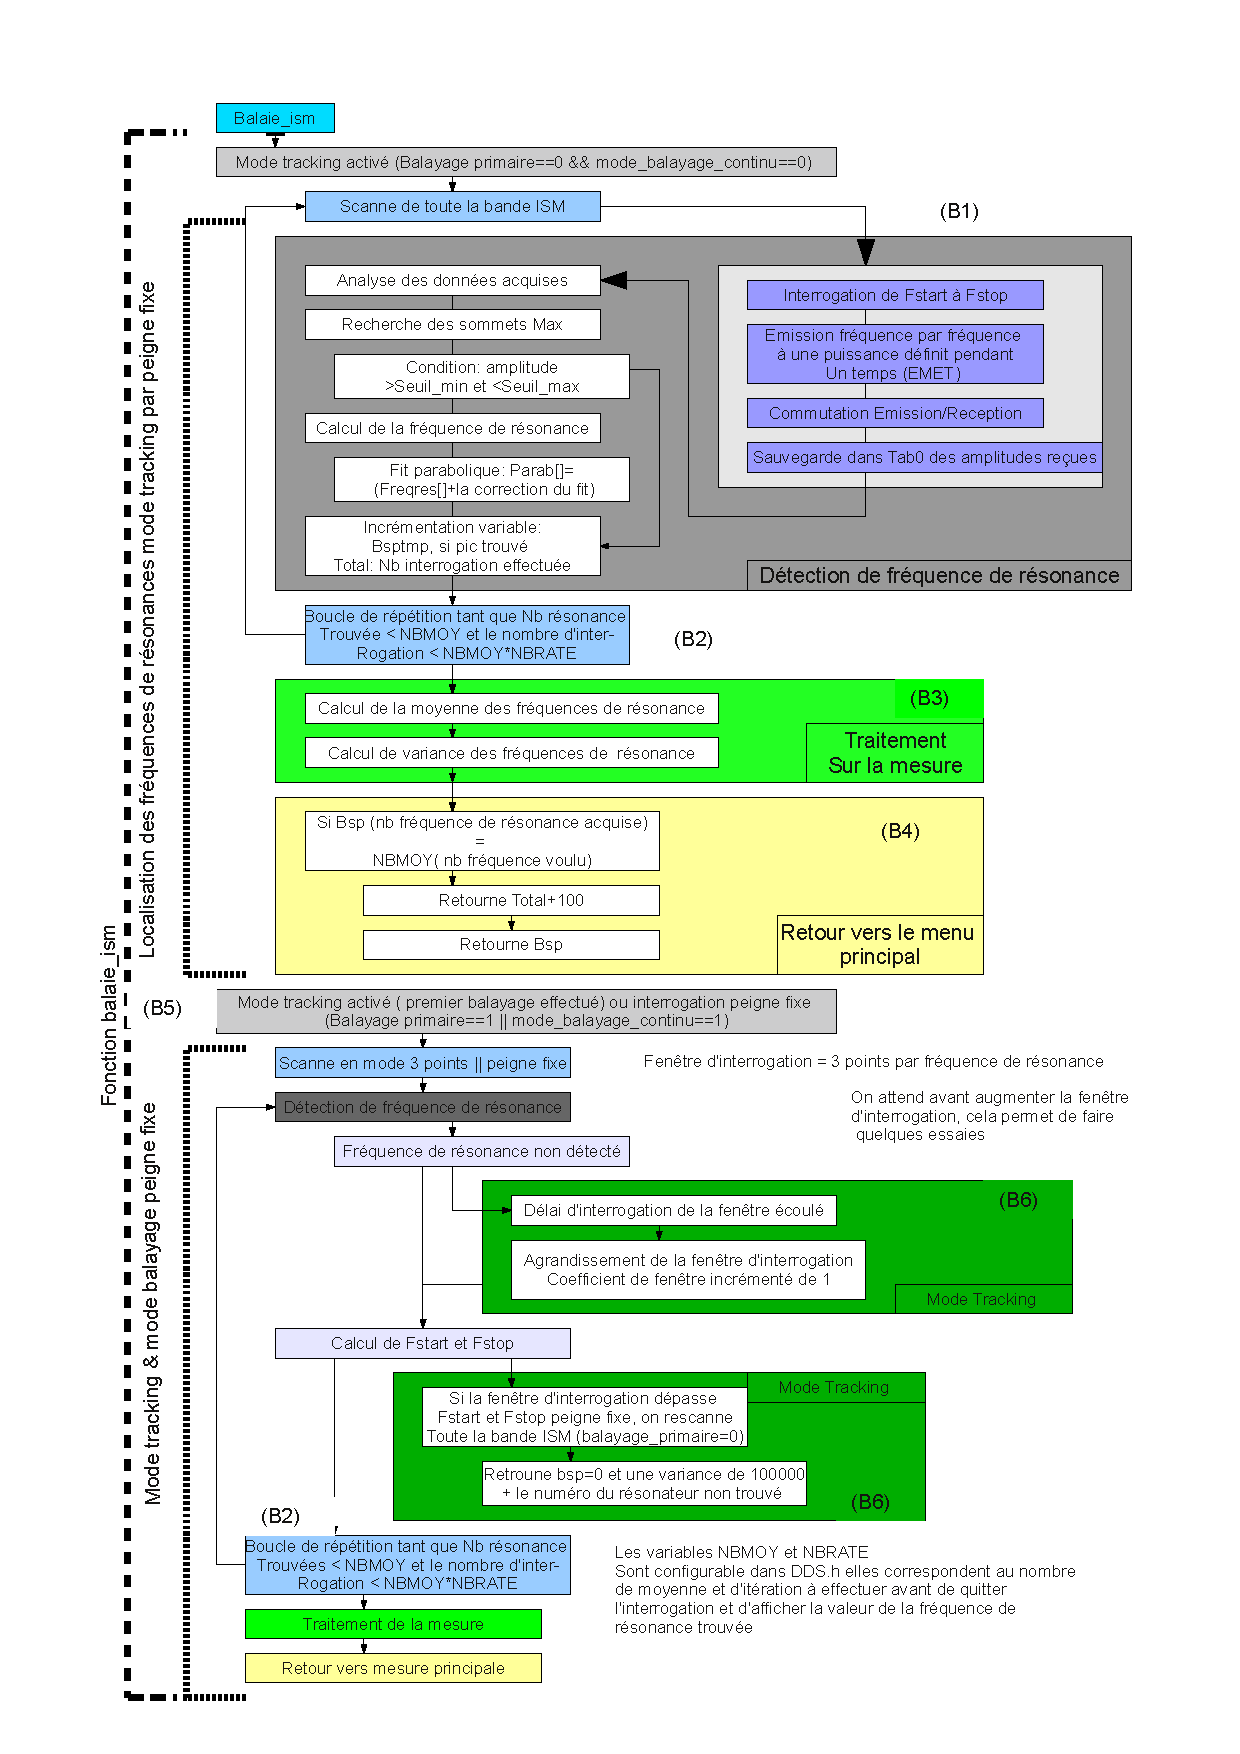
\includegraphics[width=\linewidth]{algo2}
\caption{Fonction Balaie\_ ism}
\label{hw2}
\end{figure}



\section{Taux de rafra\^ichissement}
Interrogation de 2 r\'esonateurs:
\begin{itemize}
\item Mode tracking, NBMOY=16 Taux de rafra\^ichissement max = 45 Hz
\item Mode tracking, NBMOY=1 Taux de rafra\^ichissement max = 90 Hz
\item Mode peigne fixe, NBMOY=16 Taux de rafra\^ichissement  = 45 Hz
\item Mode peigne fixe, NBMOY=1 Taux de rafra\^ichissement  = 5 Hz
\end{itemize}
Interrogation de 3 r\'esonateurs:
\begin{itemize}
\item Mode tracking, NBMOY=16 Taux de rafra\^ichissement max = 32 Hz
\item Mode peigne fixe, NBMOY=16 Taux de rafra\^ichissement  = 3 Hz
\end{itemize}

\section{Configuration du fichier DDS.h (Fig. \ref{hw3})}

Dans le fichier de configuration ''DDS.h``, nous pouvons configurer plusieurs param\`etres:
\begin{itemize}
\item L'offset : OFFSET 0xDDD0000 
\item Mode de debuggage qui permet de voir le d\'eroulement du programme #define debug
\item Controle automatique de puissance  agc=1;
\item Nombre de moyenne NBMOY=16;
\item Nombre de r\'esonateur NBPICS=2; 
\item Nombre de pas par bande NBSTEPS=(64) 
\item Nombre d'antenne ANTENNES=1;
\item Mode tacking/peigne fixe mode\_ balayage\_ continu=1;	  
\item Nombre de r\'esonateur d'une grandeur physique  PRESSION
\item Nombre de r\'esonateur de l'autre grandeur physique TEMPERATURE
\item Nombre de r \'ep\'etition de la mesure de la premi\'ere grandeur NB\_ REPETITION
\item Borne de fr\'equence de start Fintsta[NBPICS\_ MAX]=${0x28F5C200,0x2CCCCC00,0x2E147AE0};$
\item Borne de fr\'equence de stop Fintsto[NBPICS\_ MAX]=${0x2CAC0800,0x2E147AE0,0x2F5C2800};$
Pour avoir un mesure valide, nous devons voir tous les capteurs de la grandeur PRESSION ou tout les capteurs de la grandeur TEMPERATURE.
La somme de (PRESSION + TEMPERATURE)=( NB\_ PIC\_ MAX )=(NB\_ PIC). Si nous avons un capteur de temperature constitu\'e de 2 r\'esonateurs avec 
un capteur de pression constitu\'e d'un r\'esonateur, on a PRESSION = 1, TEMPERATURE = 2, NB\_ PIC=3, NB\_ PIC\_ MAX =3.
\end{itemize}

\begin{figure}[h!tb]
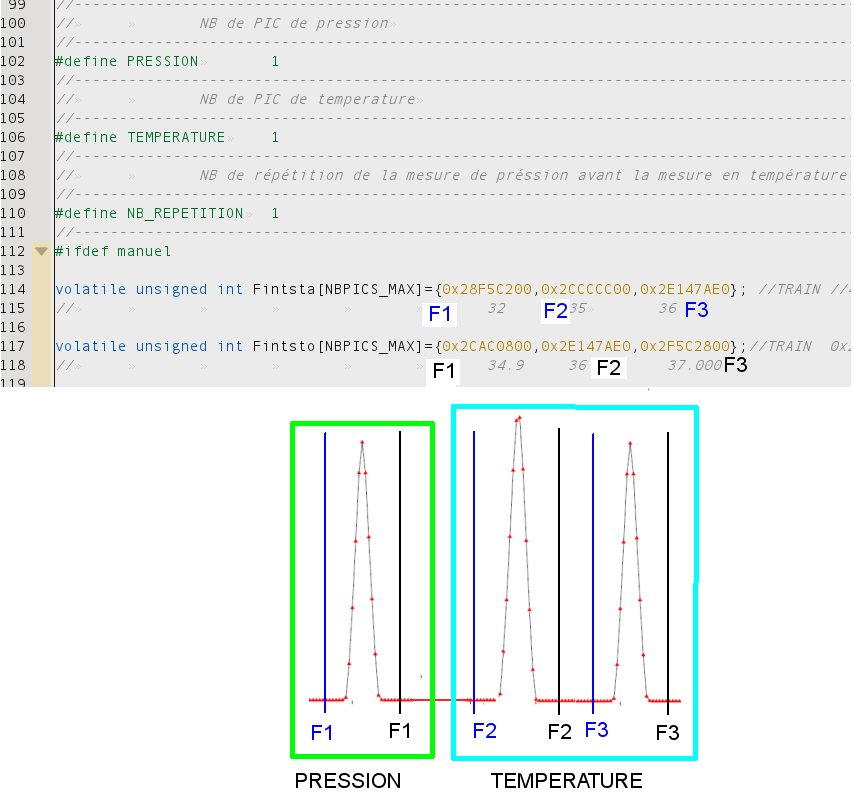
\includegraphics[width=\linewidth]{DDSH}
\caption{DDS.h}
\label{hw3}
\end{figure}

\section{D\'ebuggage et affichage des donn\'ees}
Pour \'eliminer les fr\'equences  erron\'ees, nous pouvons filtrer :
\begin{itemize}
\item Avec une hauteur Max/min d'amplitude d\'etect\'ee
\item Avec une variance faible, si la variance est \'elev\'ee, c'est que nous avons des perturbations. Si elle est de 100000, 100001... Nous n'avons 
pas r\'eussi \`a trouver le r\'esonateur 1,2... en mode tracking.
\item Le nombre BSP  correspond au nombre de valeur trouv\'ee si il est $<$ \`a NBMOY sinon il correspond au nombre d'interrogation total r\'ealis\'e 
quand nous avons r\'eussi \`a avoir NBMOY fr\'equence de r\'esonance.

\end{itemize}


\end{document}
